\documentclass[12pt, a4paper, openany, twoside]{book}
\usepackage[italian]{babel}
\usepackage[T1]{fontenc}
\usepackage[utf8]{inputenc}
\usepackage{amsmath} 
\usepackage{xcolor}
\usepackage[margin=1in]{geometry}
\usepackage{graphicx}
\usepackage{hyperref}
\graphicspath{{./img/}}
\hypersetup{
colorlinks=true,
linkcolor=blue,
filecolor=magenta,      
urlcolor=cyan,
}
%usepackage[latin1]{inputenc}
\begin{document}
\pagestyle{headings}
\author{DaveRhapsody}
\title{Reti e Sistemi Operativi}
\date{3 Ottobre 2019}
\maketitle
\tableofcontents
\chapter{La rete}
La rete è un insieme di nodi, che sono tendenzialmente pc, server, terminali,
e dispositivi radio che consentono ai dispositivi senza fili di collegarsi
(per intenderci, gli access point wi-fi), ma attenzione! \\ \\
Qui si parla di wi-fi, non della rete a cella telefonica, non si parla di 4G etc.
\section{Il modello TCP/IP}
Al centro è presente un Router, dispositivo in grado di INDIRIZZARE quelli che
sono i pacchetti IP (Internet Protocol). Cos'è un pacchetto?
\paragraph{Pacchetto}: E' un "Record/Struct" composto da un campo dati 
detto payload), ed un
campo header, che serve al protocollo di riferimento come etichetta che dice (ad 
un protocollo)  "Questo pacchetto lo puoi leggere".
Cosa contiene l'Header? 
$$header=\begin{cases}
indirizzi \\ livelli~di~priorità \\ contatori 
\end{cases}$$
A che servono i contatori? 	\\
Immagina di avere un problema nella rete in cui appare un routing loop (pensate
alla lista circolare)\\ \\
I pacchetti è auspicabile che siano di dimensioni piccine, immaginate un film 
di dimensioni tendenti al Gigabyte, un pacchetto da un Giga è pressochè (ad oggi)
insostenibile, pertanto, si riduce in pezzettini. Soprattutto c'è una probabilità
di errore più bassa! 
(Pensate di mangiarvi una Fiorentina in un solo boccone o di tagliarla prima un
pochino, stesso concetto.) \\ \\
Un altro motivo per cui vengono usati i pacchetti è legato al fatto che inviare
un qualsiasi dato occupa un canale. Intendiamoci, se da A a B (terminali) abbiamo un solo
cavo, non c'è problema, no?	\\ \\ Ok, ma se A e B sono degli switch aventi 10 pc 
connessi assieme? Se uno deve caricare un giga di roba la gente deve aspettare 
che questo finisca MA utilizzando un sistema a pacchetti, otteniamo che ci sia
una sorta di "turno" per ogni pacchetto. Di conseguenza non si intasa la luce.
\\ \\
Il sistema sopracitato si chiama multiplazione o multiplexing statistico, perchè
quando io metto tanti flussi di info che viaggiano sullo stesso collegamento, 
potrebbero accadere congestioni di rete, oppure comunque uno deve aspettare. Ecco
i pacchetti dei pacchetti che attendono si chiama buffer. Più hai host di rete,
più ti conviene aumentare la dimensione del buffer.
\\
\paragraph{Lo switch} Sono dei dispositivi che consentono di costruire la rete
con più livelli, proprio perchè ad essi vengono collegati altri dispositivi. 
Uno switch utilizza connessioni Ethernet, ed una serie di nodi collegati ad uno
switch forma una LAN. ATTENZIONE, quando si menziona l'access point, la rete 
che si forma si chiama WLAN, ovvero (Wireless LAN (Local area network)).
\paragraph{Terminale}
Il terminale (o host) sarà tendenzialmente un qualsiasi dispositivo che hosta 
applicazioni che lavorano in rete. 
\subparagraph{ATTENZIONE} la rete è identificata dal Router.
\\
Quando noi diciamo Internet, di fatto, stiamo parlando di un insieme di reti,
appunto inter - net, più reti, ergo, più router. C'è un agreement totale che 
consente ad un terminale in una zona, per poter arrivare ad un'altra.
\\ \\
Vi ricordate il cammino dei nodi? Ecco, stesso concetto.
\\
Questi nodi che si attraversano per passare da una rete A ad una rete B si 
chiamano autonomous systems, ed il cammino tra mittente e destinatario di un 
messaggio è identificato dagli autonomous per cui il pacchetto passo.
\\ \\
Più precisamente questi Autonomous sono dei Gateway, gestiti con un protocollo
(BGP, Border Gateway Protocol) in grado di regolare le comunicazioni tra questi AS.
\\ Ogni sistema autonomo, a sua volta all'interno avrà un certo insieme di altri 
router e reti, e quindi sarà presente un altro protocollo (IGP, Internal gateway 
protocol).
\paragraph{Sicurezza di un AS}
Ogni sistema autonomo è gestito da un "master" in grado di poter decidere cosa 
possa passare da quella rete, specifica le famose policy di Routing. La domanda
che sorge è.. Chi gestisce gli AS in toto? I gestori della rete, quelli telefonici.
\section{Cosa influenza le prestazioni di una rete?}
Analizzeremo due quantità
\paragraph{Latenza/ritardo}
La latenza (o ritardo) non è altro che il tempo che intercorre tra l'invio e la 
ricezione di un pacchetto. 
Esistono diversi tempi:
\begin{itemize}
	\item Tempo di processing: E' una quantità infinitesimale che indica il 
	tempo impiegato per elaboare un pacchetto
	\item Tempo di coda: Per misurarlo devo capire oggettivamente quanto viene
	usata quella coda (esistono interi studi sulle code, ma a noi ci importa
	una bellissima  ;) (Almeno, per questo corso si intende)) \\ \\
	Per un sistema stabile è auspicabile che il rapporto tra i dati contenibili
	nel buffer ed il rate di dati trasmessi al secondo sia $\leq$ 1, detto meglio:
	$$ \frac{nL}{R}\leq 1$$ 
\end{itemize}
\paragraph{Throughput}
Il through put è il quantitativo di dati che riescono ad essere trasferiti in 
un determinato quantitativo di tempo (Avete presente Mbps, Gbps, Kbps, quella
roba lì)
\section{Stratificazione}
Il concetto di stratificazione consiste nel includere le funzioni di una rete
non in un solo protocollo ma in una serie di protocollo che abbiano uno
specifico compito, e sia indipendente dagli altri 
\paragraph{La filosofia KISS}
Keep it simple stupid, è la filosofia che regola anche il mondo Unix e Gnu/Linux,
ovvero, ogni componente fa il suo mestiere, fa la sua funzione, evitare di 
mettere in mano ad un componente 10 compiti diversi, per intenderci. 
\\ \\ 
Inoltre dividendo in più componenti io ho possibilità di testare il singolo
componente, il singolo protocollo, il singolo problema SENZA, S E N Z A andare
a danneggiare o danneggiare gli altri protocolli/componenti!
\paragraph{Stack ISO/OSI}
Questo è lo stack più preciso ingrandito dell'TCP/IP, visto dal livello più 
basso al livello più alto
\begin{itemize}
	\item physical
	\item data link
	\item network
	\item transport
	\item session
	\item presentation
	\item application
\end{itemize}
\section{livello Physical}
Nel livello fisico viene convertito quello che è il segnale elettrico in una
sequenza di 0 ed 1
\section{Livello Data Link}
Si implementa MAC (Medium Access Control), converte quelli che erano
degli 0 ed 1 e li fa diventare dei pacchetti (yes, c'è il primo header, cioè 
quello del physical).
\\ \\ 
L'indirizzo MAC identifica univocamente un dispositivo in rete, QUALSIASI esso sia.
E non solo, mondialmente, N O N esistono due dispositivi DIVERSI aventi lo STESSO
Mac address. A che serve oltre questo? Serve al protocollo ip per capire CHI
è il mittente o destinatario, e sì, è incluso nell'header
\section{Rete} E' il livello di internet, l'IP protocol, con indirizzo ipv4 v6 etc.
\section{Trasporto}
E' il livello in grado di trasportare tramite internet quelli che sono i pacchetti
applicazione, trasporta i datagram ip, trasporta i pacchetti appunto tramite 
internet, sono presenti due protocolli (TCP e UDP) che si occupano di fare questo
\section{Applicazioni} Il nome parla da sè, non lo studieremo in questo corso.
\\ \\
Qui noi si studierà dal data link al transport MA in ordine invertito, ovvero
partiamo da "Che cosa vuole l'applicazione?" e poi andiamo a scalare.
\paragraph{Precisazione:}
Dato un pacchetto in un qualsiasi livello (escluso lv application), 
quando viene aggiunto l'header, il nuovo pacchetto potrà esser letto SOLO dal
protocollo del livello superiore! \\ \\
Su questo stesso piano, se ho un pacchetto con già l'header aggiunto, questo
potrà essere spacchettato SOLO da un protocollo del livello inferiore.\\ \\
Ogni livello offre servizio al livello immediatamente superiore od inferiore in
base al verso del flusso dati.
\\
{\color{black} \rule{\linewidth}{0.2mm} }
\paragraph{La magica teoria (o ricetta) dell'incapsulamento di Dave} 
Per spiegare meglio cosa accade, immaginatevi una fetta di prosciutto, bene, 
questa fetta di prosciutto rappresenta il \color{red}flusso elettrico\color{black} che vien gestito 
dal livello fisico. \\
A questo punto, immaginatevi due fette di pane che si chiudono sulla fetta di 
prosciutto. Benissimo, il Data Link ha \textbf{INCAPSULATO} il prosciutto ed ha
creato un panino (\color{red}Pacchetto\color{black})! \\ \\
Il data link passerà questo panino al \color{red}Network \color{black}, e lì ci 
saranno altre due fette di pane che includeranno il nostro panino. 
Ed in questo modo abbiamo ottenuto un panino dentro ad un altro panino! Ossia,
un pacchetto incapsulato in un pacchetto che semplicemente aggiunge un header 
(o intestazione) ;) Ma torniamo seri adesso. \\
\href{https://www.youtube.com/watch?v=6HHe1AIUMM4}{Premete qui per vedere un
video corso che spiega con precisione l'incapsulamento.}
\\
{\color{black} \rule{\linewidth}{0.2mm} }
\\
\chapter{Livello Trasporto}
Il livello di trasporto è il livello che riceve messaggi dal livello application
ed ha come compito quello di mettere in comunicazione end-to-end due nodi.
Nel caso del livello di trasporto non si parla di pacchetti ma di Segmenti (
Dall'esempio sopra riportato sì, è stato incapsulato il pacchetto del lv network).
\\ \\
Quando viene analizzato il segmento si effettua la DEMULTIPLAZIONE 
(Demultiplexing), ovvero si analizza l'header del segmento per vedere a quale
applicazione sarà destinataria di un determinato messaggio.
\paragraph{Cosa contiene un segmento di trasporto?}
\begin{itemize}
	\item Numero di porta: presente in ogni segmento, rappresenta una applicazione
	e dal punto di vista dell'applicazione è come se fosse un punto di 
	accesso, detto anche SOCKET. 
	\paragraph{NON CONFONDIAMOCI} Il livello transport vede una porta, mentre
	il livello applicazione vede un socket. All'atto pratico c'è una syscall
	che letteralmente può attivare qualsiasi socket.
	\item Protocollo Transport TCP o UDP.
\end{itemize}
\paragraph{Che differenza c'è tra TCP e UDP?}
UDP è quello che usate negli streaming di Rojadirecta
, in cui pur di vedere la vostra squadra 
(che ovviamente è la Fiorentina, vero? <3) non vi preoccupate di perdere qualche
dato (tipo immagine un po' sgranata ogni tanto e simili).
\subparagraph{Infatti} UDP se ne frega se un pacchetto è arrivato, è usato
per comunicazioni anche per esempio le voice chat, roba di questo genere, poichè
\textbf{NON} effettua alcun controllo sulla correttezza dei messaggi, diciamo
che lui ti invia roba, se non ti arriva non gli importa, va avanti, perchè qui
è importante che si sia il più aggiornati possibile.
\\ 
Al contrario TCP effettua questi controlli, perchè con TCP si garantisce la 
correttezza (sia dei dati stessi che dell'ordine in cui arrivano), pertanto 
potrebbe essere un problema.
\\ \\
Il segmento può avere sia TCP che UDP, e nel caso di UDP si ha un IP +
Porta di destinazione, o meglio
$$Pacchetto UDP~ =~ \begin{cases}
SourcePort: ~Porta~ sorgente \\
DestinationPort: ~Porta~ di ~destinazione \\
Lunghezza: Indica~ la~ lunghezza ~totale ~del ~segmento~ (+payload~ \\dei ~livelli
~inferiori)\\
Checksum:~ Verifica ~la ~correttezza ~di ~trasmissione \\
\end{cases}$$
\\ 
Supponiamo di avere un web server, (quello che consente di vedere una pagina web)
, la porta d'accesso è la stessa ma hai più utenti con la stessa pagina
\\ \\
Nel caso di TCP invece un segmento è composto non solo dall'IP + la porta di 
destinazione, ma è composto in questo modo:
$$\begin{cases}
IP_{A} \\
IP_{B} \\
PORT_{A} \\
PORT_{B}
\end{cases}$$
A e B in questo caso sono tendenzialmente sorgente e destinataria, ed il calcolo
del checksum precedente è effettuato direttamente dal livello Transport stesso.
\\ \\
Attenzione, nell'introduzione abbiamo anche detto che già nel datalink abbiamo 
dei controlli, pertanto ogni livello può svolgere la correzione dei pacchetti,
pertanto non si attiva quasi mai, perchè Transport dà per scontato che Network
e Datalink gli abbian passato qualcosa di corretto.
\\ \\
Il codice di implementazione del controllo è tipo di migliaia di righe di codice
per correggere o prevenire errori, ed è giustissimo così. Contiamo che ormai TCP
e UDP non si possono rompere, sono più che sicuri.
\section{TCP}
Il concetto è che si vuole trasferire dati in modo affidabile, o meglio, si 
vuole fare in modo che i dati arrivino a destianazione 
e siano corretti in generale.
\\ \\ 
Il trasferimento dati affidabile dipende da una serie di fattori, e si verifica
quando ho una rete con le seguenti caratteristiche:
\begin{enumerate}
	\item Nessuna perdita
	\item Nessun errore
	\item I dati son corretti e presenti tutti quanti
\end{enumerate} 
\paragraph{Nel caso avvengano errori} si può ricorrere a diverse metodiche di
soluzione, come ad esempio la tecnica di ritrasmissione. Ossia, non ti è 
arrivato il mio pacchetto? Ok, te lo rimando. Nell'atto pratico è una cosa del tipo
$$\begin{cases}
if(ricevoAcknoledgment)~then~mandoSucessivo(); \\
else~if(ricevoNotAcknoledgment)~rimandoPacchetto();
\end{cases}$$
Quello che chiamo not acknoledgment (che da ora chiameremo solo ACK) viene 
inviato SE il pacchetto è non corretto, per esempio per il checksum.
\\ \\
E se il pacchetto poi è lo stesso? Ne ricevo due? No. I pacchetti sono numerati
hanno un ordine, pertanto
$$\begin{cases}
if(ricevoACK) m+1;\\
else m
\end{cases}$$
con m che è il "pezzetto" successivo o precedente, è importante che si capisca 
questo.
\\ \\ Ora cerchiamo di integrare, è necessario che il sistema mi mandi indietro
sì se ha ricevuto ma ANCHE la posizione a cui è arrivato! (Sistema PAR, positive
acknoledgmente with retransmition).
\\ \\
Quindi mi mandi un messaggio e io ti rispondo dicendo ok messaggio, tu mi mandi
il due, io rispondo ok due, tu mi mandi tre io rispondo ok due, mi rimandi tre.
\paragraph{Perdite}
Sì, ok, ma se uno non mi riesce a rispondere? Si imposta un semplice timer
la cui scadenza implica che ti rimando il pacchetto. Un po' come quando dici
una cosa con la musica alta a uno e lui ti guarda tipo fisso... Passa tempo, e
poi ripeti la cosa. 
\\ \\ 
E se io continuo a rispondere? Lui che fa continua come un pazzo a ripetere la
stessa cosa come Ciuchino che chiedeva a Shrek ogni 2 millisecondi
"Siamo arrivati?"? NO! C'è un contatore che si aziona ad ogni mancata risposta,
una volta che arriva ad un tot, chiudo la comunicazione.
$$\begin{cases}
if(timerGoesOff) ~ trasmetti(messaggio_{i}) ~ AND ~ setTimer(0); \\
else ~if(ACK_{i}) ~trasmetti(messaggio_{i+1} ~ AND~  setTimer(0)); \\
else~ trasmetti(messaggio_{i}) ~ AND ~ setTimer(0);
\end{cases}$$
\paragraph{ATTENZIONE} Supponendo un timer troppo corto, accadrebbe che il 
destinatario non fa in tempo a rispondere, e quindi il mittente rifà la domanda
prima di ricevere la risposta, hai già due domande con una risposta. \\ \\ 
All'atto pratico questo problema esiste davvero, è un problema reale, pertanto si deve
riuscire a capire il modo in cui il timer vada adattato alle condizioni di rete,
che a seconda del traffico può essere più lenta o anche più veloce.\\ \\
\subsection{I tempi di una connessione}
Riprendiamo il concetto di latenza (tempo che intercorre tra invio e ricezione),
bene, quello è concettualmente il tempo di trasmissione, da qui possiamo calcolare che
$$utilizzoRete = \frac{\frac{L}{R}}{latenza+\frac{L}{R}}$$ 
in cui $\frac{L}{R}$ Ha R che è la velocità di trasferimento
dei pacchetti, mentre invece L sarebbe la lunghezza
, ossia: $\frac{L}{R} = \frac{Lunghezza}{Velocita'~trasmissione}$
E la latenza... E' la latenza. 
\subsection{Protocolli a Finestra Scorrevole (Sliding Windows)}
Io trasferisco un insieme di w pacchetti, i quali impiegheranno $w*\frac{L}{R} 
\geq \frac{L}{R}+RTT$ tempo ad esser trasposti, pertanto ne esce che
$$w \geq \frac{RTT\cdot R}{L} +1$$
Questo ovviamente in mancanza di errori e perdite.
\\ \\
\subparagraph{Osservazione:} Stiamo ragionando su sistemi concettualmente 
indistruttibili, quindi diciamo che non si è quasi menzionata la possibilità che
un host possa disconnettersi.
\subsection{Go Back N} 
Poniamo caso che io trasmetto 5 messaggi: $m_{1, ..., 5}$ e mi arriva l'ok di
ricezione dall'1 al 3, malgrado li abbia trasmessi tutti e 5, pertanto ciò che
accade è che rinvierò dal messaggio 3 in poi.
\subsection{Selective Repeat}
Traccio la vita di ogni pacchetto individualmente, ossia ritrasmetto solo il
pacchetto mancante, il problemino è legato al fatto di avere tanti timer, ma
oggi c'è da considere che abbiamo processori nell'ordine dei Ghz, no problem.
\\ \\ 
Quando all'epoca il massimo processore esistente era di massimo 10 Mhz, insomma
chiaro che ora essa sia la migliore delle soluzione. Ma cosa richiede più precisamente
l'SR?
\begin{itemize}
	\item Ack individuali per ogni pacchetto
	\item Un timer per ogni singolo pacchetto
	\item Buffer sul ricevitore (E' un array di booleani all'atto pratico)
\end{itemize}
Ci sono dei casi in cui ci sono interazioni tra numero di pacchetto e dimensione
finestra, ma sono problematiche di cui non approfondiamo perchè non ci interessa
siccome non può praticamente mai capitare
\section{Formato del pacchetto}
\begin{itemize}
	\item 20 byte
	\begin{itemize}
		\item 16 bit Source + 16 bit destination port
		\item 32 bit Sequence Number\\
		Se i numeri di sequenza contassero il numero di segmenti, pensate averne 
		$2^{32}$ E INFATTI, vengono contati in Byte, quindi il numero di sequenza fa 
		riferimento al byte
		\item 32 bit ACK Number
		\item 8 bit di cui 4 indicano l'header length e gli altri 4 son inutilizzati \\
		16 bit di recive window, ovvero quanti bit posso accettare 
		\item 16 bit di checksum + urgent data (in seguito vedremo le funzioni dei 
		vari flag)
	\end{itemize}
	\item Payload ($\chi$ Byte, perchè la dimensione è variabile, dipende
	dal carico di dati che trasporta)
\end{itemize}
Diventa ragionevole contare i Byte e non i segmenti perchè nel periodo in cui è 
nato TCP il costo per la banda di rete era elevato, quindi il singolo byte 
faceva la differenza in una trasmissione.
\subsection{Le Flag}
\begin{itemize}
	\item CWR: Congestion window reduced
	\item ECE: End to End congestion 
	\item U: Urgent Data
	\item P: Push\\
	Trasmetti senza far funzionare i tuoi algoritmi che assemblano un tot di dati.
	\item ACK: Ti dice se è un ACK
	\item RST: Reset della connessione per via di un problema nella sequenza\\
	oppure il ricevitore ti chiude la porta e non apre la connessione
	\item SYN: Sincronizzazione, semplicemente apre la connessione
	\item FIN: Chiude la connessione
\end{itemize}
\subsection{Gestione dei riscontri}
Devo inviare dei pacchetti, e quindi devo riscontrarli, come si gestisce il 
valore dei puntatori? \\ \\
A invia un messaggio con Seq = 10, ACK = 57, [ciao] stiamo intendendo un messaggio
avente questi 3 parametri principali, li possiamo mettere pure a sistema così, 
per intenderci meglio:
\[
messaggio =
\begin{cases}
Seq = 10 \\
ACK = 57 \\
[ciao]
\end{cases}
\]	
Cosa mi aspetto come risposta? Beh io sto comunicando che siamo al $57_{esimo}$
ACK e al 10 byte di sequenza, pertanto tu mi aspetto che mi si dica UEH sono
arrivato a 57 e mi risponde:
\[
messaggio =
\begin{cases}
Seq = 57 \\
ACK = 14 \\
[bella]
\end{cases}
\]	
Il concetto è che la sequenza della risposta coincide con l'ack della "domanda",
sembra sbagliato, no? Bene, se ti comunico che sono a $\lambda$ mi aspetto che
tu mi risponda che sei arrivato alla sequenza $\lambda$. Pertanto in risposta
accadrà che la sequenza dovrà coincidere con l'ack precedente. \\ \\
Se all'inizio si era al segmeto 10, verrà risposto che si è al segmento 57 MA
quando verrà inviato di nuovo si riscambia, diciamolo in modo più sensato:
\[
EstimatedRTT = (I - \alpha) \cdot EstimatedRTT + \alpha \cdot SampleRTT 
\]
Con $\alpha$ = 0,125 nella maggior parte dei casi (E' il valore tipico).
Ed rtt che sarebbe il rounded
trasmission time, cioè in parole povere il tempo che ci si impiega a trasmettere.
\\ \\
Tutto va in funzione di come cambia l'RTT nel tempo, conviene avere un RTT che 
nel tempo rimane lo stesso, non conviene avere un RTT troppo ballerino
\[
DevRTT = (1 - \beta) \cdot DevRTT + \beta \cdot | SampleRTT - EstimatedRTT
\]
Dove dev sta per deviazione (O margine di sicurezza) e tipicamente $\beta$=0,25\\
Infine definiamo quello che è il $Timeout = EstimatedRTT + 4\cdot DevRTT$
\subsection{Passo 2: Ritrasmissione}
Quando non va tutto bene potrei dovere ritrasmettere dei segmenti, perchè? 
Generalmente per via di o timeout oppure ack duplicati.
\\ \\
Il nostro trasmettitore fondamentalmente trasmette segmenti, nel caso il 
ricevitore non riceve allora questo ritrasmette, e nelle puntate precedenti si è
visto cosa può accadere (Timer e ACK duplicati), ed infine resetta il timer.
\\ \\
\paragraph{ATTENZIONE} NON esiste un preciso modo per cui possano verificarsi dei
problemi di ricezione, possono accadere miliardi di differenti inconvenienti, 
per dire anche il fatto che ti arriva un segmento a metà, l'altro solo inizio e 
fine
\\ \\
\subsection{La perdita dei pacchetti}
Se il trasmettitore invia un pacchetto che però non arriva, il ricevitore manderà
l'ack precedenti dicendo che manca un pezzo, possono esserci diverse situazioni.
(Si ok, perchè manda un altro ACK? Semplicemente perchè potrebbe essersi perso 
pure quello, non funziona una s**a in questa rete.).
\subsection{Pacchetti che arrivano non in sequenza}
Abbiamo visto il selective Repeat, ma c'è anche un altro modo un po' diverso che
ha un unico timer (soluzione che impiega più ram che processore) perchè sul 
trasmittente avremo un array di ack che dice dove e cosa è stato ricevuto. Esempio:
\\ \\
Io invio da 1 fino a 5, mi rispondi 4, io ti mando poi 6, 7, 8, allora in base a
quale elemento dell'array non risulta true io ti mando quella zona. Ad esempio ho 
true gli ack da 1 a 8 MA manca proprio il 5. Allora semplicemente mando il 5. 
OVVIAMENTE ricordiamoci che il timer è utilizzato anche in questo caso.
\\ \\
Potrebbe anche accadere di avere dei riscontri cumulativi o duplicati. Il cumulativo
è quando tu mi invii 1, 2 e 3 e io rispondo solo 3, tu dai per scontato che io abbia
ricevuto i precedenti.
\subsection{La receive Window}
In un meccanismo a finestra ho una.. Finestra in cui posso trasmettere. Cosa determina
la suddetta? In pratica controllo la quantità di dati che posso trasmettere. 
Se in capo mi entrano 3 parole al minuto durante le lezioni, e i prof ne dicono
500 leggendo le slide, ne perdo un patrimonio in una lezione, stessa cosa per 
le reti. \\ \\
Siccome in una rete è meglio evitare questo problema si implementano la ReceiveWindow
e la CongestionWindow (Finestra di ricezione e congestione), e il valore che 
dovremo assumere sarà $W = min\{CongWindow, RcWindow\} $, ricordando sempre la
formula che la dimensione dei pacchetti da trasmettere è $\frac{W}{RTT}$
\\ \\ 
\section{Inizio della connessione: HandShake a 3 vie}
Handshake vuol dire letteralmente stretta di mano, tipo saluto, prendiamo
per presupposto di avere due host che chiamiamo A e B \\ \\
Questi non si conoscono, pertanto A manda a B un messaggio con
\[
A ~ scrive: \begin{cases}
SYN \\
Seq = \kappa \\
[]
\end{cases}
\]
\[
B ~ risponde: \begin{cases}
SYN \\
Seq = \psi \\
ACK = \kappa + 1
[] 
\end{cases}
\]
Che tradotto in termini pratici è tipo:	\\
A: OH INIZIO A $\kappa$
B: OH HO RICEVUTO $\kappa + 1$, IO SONO A $\psi$
\[
A ~ replica: \begin{cases}
SYN \\
ACK = \psi + 1
[] 
\end{cases}
\]
Che è traducibile in "OK HO RICEVUTO $\psi + 1$"
\section{Fine della connessione}
\[
A ~ scrive: \begin{cases}
FIN \\
Seq = \kappa \\
[]
\end{cases}
\]
\[
B ~ risponde: \begin{cases}
FIN \\
ACK = \kappa + 1
[] 
\end{cases}
\]
Se però B non ha ancora finito, allora gli manda solo un ACK, mentre
se ha finito anche lui, semplicemente si chiude la connessione
\section{Congestione di rete}
Avviene nel momento in cui viene inviata una quantità di pacchetti SUPERIORE a 
quella che normalmente può essere ricevuta, che è come quando ad Analisi venivano
scritte troppe cose alla lavagna e non si riusciva a starci dietro, prima o poi 
avvengono perdite di dati. \\ \\
Per evitare le congestioni ci sono una serie di meccanismi. Perciò iniziamo a 
definire una nuova quantità: MSS = Maximum segment Size, ovvero dimensione massima
di un segmento.
\subsection{AIDM: Additive Increase Mult. Decrease}
Invio un messaggio, tu rispondi ok, poi ne mando due, rispondi due, poi tre e 
rispondi tre. Progressivamente cresce la finestra, arriverò ad un valore $\lambda$
per cui non riesci a rispondere e c'è una perdita, ma può esser di due tipi:
\begin{enumerate}
	\item Loss: Perdita
	\item Timeout: Ci impiego troppo tempo a passare tutto
\end{enumerate}
Il peggio tra i due è il timeout, perchè manca proprio una risposta, mentre 
se ho delle perdite almeno c'è comuniazione! Perciò cosa succede, appena c'è una
perdita viene dimezzato il numero di dati che invio. Se la prima perdita si verifica
a $\delta$ allora ripartirò da $\frac{\delta}{2}$.
\\ \\
Notiamo subito che questo metodo è estremamente lento, perciò c'è un secondo 
metodo che fa la stessa cosa ma invece di incrementarsi di uno si incrementa 
esponenzialmente (1, 2, 4, 8 ,16, 2$^{n}$)
\\ \\
Questo meccanismo esponenziale si chiama Slow Start e funziona allo stesso modo
poi per quando si dimezza tutto.
\\
Quello che abbiamo visto è come fare per trovare la quantità di dati massima 
che è possibile trasmettere SENZA PERDITE.
\paragraph{Come si gestisce il timeout?} 
In questo caso va abbassata di tanto la finestra, perchè in questo caso non 
viene nemmeno ricevuto il pacchetto, scade il timeout ancor prima di aver 
rimandato indietro il pacchetto perciò come si agisce? \\ \\
Il funzionamento è identicop a quello per la perdita di pacchetti, si ragiona
incrementando esponenzialmente il numero di pacchetti, poi si arriva al timeout,
si dimezza, e si riparte da lì MA questa volta incrementando di 1 alla volta.
\\ \\
Questo incremento di un'unità per volta viene chiamata Congestion Avoidance, e
(come da nome) va a risolvere le congestioni.
\paragraph{Ok, ma perchè non fare direttamente 1 alla volta?} Perchè il tempo
è una risorsa essenziale, e ragionare di pacchetto in pacchetto richiederebbe
troppe risorse, semplicemente in questo modo si risparmia tempo, tutto lì.
\chapter{Sistemi operativi}
Un sistema operativo è un software, un programma, che agisce da intermediario
tra l'utente ed il suo computer.\\ \\
Molto semplicemente anche solo per scrivere questi appunti, e voi per visualizzarli
stiamo usando un sistema operativo. Ma andiamo per livelli
\begin{enumerate}
	\item Utente: Esseri umani, OPPURE anche altri computer, l'utente può essere
	qualcuno o qualcosa che necessità l'intervento del computer fondamentalmente.
	\item Applicativi/Application programs: Sono il software applicativo, nel 
	senso che si applicano per risolvere un problema pratico, ad esempio per dire
	programmi di editing foto, oppure il browser, cioè fondamentalmente estendono
	le funzioni fattibili dalla macchina
	\item \color{red} Sistema operativo  \color{black}: Controlla e gestisce
	l'hardware al servizio dei nostri applicativi, fa appunto come si diceva da 
	intermediario
	\item Hardware: Ci si rifà al modello di Von Neumann, CPU Ram e I/O, sempre
	lì si ritorna, tutte li risorse messe a disposizione dalla ferraglia per 
	intenderci 
\end{enumerate} 
Perchè non vogliamo che gli applicativi usino direttamente l'hardware ma ci 
spariamo sopra un OS che gestisca? Per due aspetti.
\begin{enumerate}
	\item Da un lato astrae le risorse hardware, presentando una macchina estesa
	più facile da programmare (Files invece di blocchi di dati)
	\item Dall'altro, gestisce le risorse hardware del computer, assegnandole ai 
	programmi in maniera equa ed efficiente e controllando che questi le usino
	correttamente
	\begin{itemize}
		\item Nasce dalla necessità di eseguire più programmi per più utenti
		sulla stessa macchina
	\end{itemize}
\end{enumerate}
\section{Storicamente}
Per quanto concerne l'hardware rimangono buone tutte le varie nozioni ricevute
ad Architettura degli Elaboratori, lì sono state approfondite meglio da questo
punto di vista (giustamente.)\\ \\
Il sistema operativo oggettivamente fa in modo che le risorse dell'hardware
siano gestibili per eseguire più di un software alla volta sul pc, perchè di fatto
alla volta si esegue un solo programma MA ci vien data l'impressione che siano
più di uno alla volta. \\ \\
L'esigenza di gestire le risorse è nata assieme ai primi computer fondamentalmente,
quelli a valvole termoioniche, CIOE' OH SON DELLE LAMPADINE UN PO' PARTICOLARI.\\
Come già avrete sentito almeno 200 volte, i primi computer, aventi un miliardesimo
della potenza di calcolo di un nostro smartphone, eran grandi quanto una stanza,
e venivano programmati direttamente staccando e attaccando i cavi in base a cosa
si dovesse fare... Immaginatevi me a prendere gli appunti saltando da una parte
all'altra per attaccare e staccare spine. Altro che jogging e palestra.
\\ \\
Solo che le valvole si guastavano, era più il tempo per ripararli che quello per
usarli MA eran 20000 mila volte più veloce di fare i calcoli su C A R T A. 
(Computer's rules)
\\ \\
Dopo l'invenzione dei transistor i computer diventano più affidabili, inoltre,
i transistor non si fulminano, son più rapidi, 10 volte più piccini delle valvole.
Insomma, progressivamente i computer son diventati più piccini, veloci, e meno
costosi (pensate agli smartwatch tipo MiBand per intenderci).
\\ \\
In seguito all'aver capito che programmare usando spine è un po' difficoltoso, 
tipo mezza giornata per fare a = c + b, per intenderci, allora si è iniziato
a programmare con l'elaborazione \textbf{batch}, con programmi monitor per il 
caricamento ed esecuzione dei job (job control languages), (qua già si usavano
le schede perforate), e qui nascevano i linguaggi ad alto livello.
\\ \\ 
Progressivamente poi c'è stato il passaggio ai circuiti integrati, infatti
IBM con la magica linea 360 cerca di avere un'unica linea di computer adatta 
sia per ditte commerciali che per calcoli scientifici E NON SOLO perchè avevan
creato dei computer che potessero essere compatibili tra loro ma differivano
per la capacità di calcolo \\ \\
Ci son due problemi
\begin{enumerate}
	\item Lo stesso software doveva funzionare su tutti i computer della linea
	\item Occorreva gestire le risorse della macchina in maniera efficiente in 
	tutti gli scenari applicativi
\end{enumerate}
\section{Tecnica Multiprogrammativa}
Molti programmi caricati in memoria contemporaneamente, che tradotto significa 
che quando un programma è impegnato nell'i/o il processore passa ad eseguirne
un altro
\section{Spooling}
L'I/O viene spostato in un buffer in autonomia dal processore, perchè appunto
il processore interagirà con il buffer (si fa prima) anzichè con la periferica.
(Le code di stampa sono un ottimo esempio)
\section{Time Sharing}
Ad ogni persona veniva fornito un terminale ed una stampante, in cui il terminale
è rimasto, era una shell su cui tendenzialmente poteva essere eseguito bash, ma
non necessariamente, potrebbe essere stata qualsiasi shell. \\ \\
La figata sta nel fatto che con lo stesso hardware tu avevi più terminali, che
ti facevano sembrare di avere il computer solo per te ma invece era un solo
computer con più terminali. \\ \\ 
Però attenzione, poniamo di avere 10 terminali, se uno di questi fa crashare
la macchina, tutti gli altri 9 crashano, e infine se le periferiche devono
essere gestite in maniera che quando la periferica opera il processore non 
aspetta, nasce il concetto di interrupt \\ \\
L'interrupt è un messaggio della periferica che letteralmente prende la cpu, la
ferma e dice "Fermo, parlo io".
\section{La varietà di esigenze}
Esistono vari tipi di computer:
\begin{enumerate}
	\item Laptop, pc, tablet: Mi rifiuto di spiegarvi cosa sono, tenete solo
	a mente che in teoria è massimo una persona per volta (prendetevi una 
	qualsiasi Distro di linux, installateci l'ssh server e vedete che anche un 
	laptop diventa server)
	\item Server, mainframe, sono delle macchine con capacità di calcolo elevate
	(No, nel caso di un server non è obbligatorio) che rendono equa la 
	condivisione delle risorse tra molti utenti
	\item Dispositivi mobili: Avete presente i computer grandi una stanza? Ecco
	quelli sono CHIARAMENTE dei dispositivi TASCABILI mobili, no? Va beh, 
	semplicemente hanno bassi consumi energetici e buona connettività.
	\item Sistemi embedded: Funzionano senza (o con minimo) intervento umano, e
	soprattutto in tempo reale (Arduino, sì, quello è un sistema embdedded per 
	intenderci)
	\begin{itemize}
		\item ATTENZIONE, in tempo reale significa che ci son dei tempi massimi
		entro cui bisogna fare le cose, e non si può sforare quei tempi, non è
		che lavorano necessariamente velocemente.
	\end{itemize}
\end{enumerate}
\section{Composizione del Sistema Operativo}
Un sistema operativo non è un singolo programma ma è composto da una serie di 
parti:
\begin{itemize}
	\item Kernel: Software sempre in esecuzione che fornisce tutti i software
	di gestione dell'hardware (cpu ram hdd ecc)
	\item Programmi di sistema: E' una serie di software di gestione di processi
	jobs, interfacce grafiche, cose così
	\item Middleware: Servizi di alto livello per programmare applicazioni 
	(Framework grafici, sonori, etc)
\end{itemize}
\chapter{I processi}
\begin{itemize}
	\item Cos'è un processo
	\item Come vengono schedulati?
	\item Che operazioni si possono effettuare sui processi?
	\item IPC (Memoria condivisa, message passing)
	\item Comunicazione in sistemi client-server
\end{itemize}
I più attuali OS sono in grado di eseguire più software in concorrenza, allo 
stesso momento, per intenderci. Ma iniziamo a definire meglio questo software,
che da quando va in esecuzione prenderà il nome di \textbf{processo}.
\\ \\
Come si compone un processo? 
\begin{itemize}
	\item Stato dei registri del processore, compreso il PC
	\item Codice del programma (Segmento text) \\
	Sarebbe quello che buttavamo nel text di Assembly su QTSpim, cioè 
	l'insieme di istruzioni che vengono eseguite
	\item Stack delle chiamate, contenente parametri, variabili locali ed il
	return address
	\item La \textbf{Data Section} contiene le variabili globali, quelle statiche
	che vengono allocate prima dell'esecuzione dei programmi
	\item L'heap, che contiene la memoria allocata dinamicamente durante
	l'esecuzione, quella che in Java si usava quando venivano instanziati gli
	oggetti, o i vettori.\\ 
	\item Altre risorse acquisite dall'OS, come socket oppure file contenuti sull'OS.
\end{itemize}   
\paragraph{ATTENZIONE: }
Finora si è sempre menzionato il concetto di programma, sappiamo cos'è, no? 
Un programma è un insieme finito di istruzioni, fondamentalmente, ma quando
queste vengono eseguite diventano un PROCESSO.\\ \\ Il file eseguibile è un 
programma, non un processo, mentre l'applicativo che state usando ora per
leggere queste righe (Perchè son certo che non ve le stamperete su carta come
me ;) ) è un processo che avete in memoria da qualche parte. 
\\ \\
\paragraph{Come è organizzata la memoria di un processo?}
\[
\begin{cases}
stack \\
\downarrow \\
... \\
... \\
\uparrow \\
heap \\
data \\
text
\end{cases}
\]
Tra stack ed heap perchè ci sono i puntini? E le frecce? Stack ed heap 
condividono lo stesso spazio di memoria, MA cambia il verso di allocazione
dei dati. \\ \\
Lo stack inizia dall'ultima locazione di memoria, e prosegue verso il basso,
mentre l'heap inizia da dopo il segmento data. Per cui siccome condividono
memoria, nel caso se ne avesse poca, bisognerebbe prestare bene attenzione
a come questa viene usata. \\ \\
\section{Gli stati di un processo}
I processi sono in esecuzione, fin qui ci siamo, ma dove? Sull'OS. Pertanto,
la gestione dei processi è tutta opera dell'OS, e questa gestione fa la 
differenza tra un OS valido ed uno meno valido, insieme ad altri fattori.\\ 
\\
Gli stati di un processo sono:
\begin{itemize}
	\item New: Il processo è in attesa di essere ammesso (admitted) dallo
	scheduler
	\item Ready: Il processo è stato schedulato ed è pronto per essere 
	eseguito 
	\item Running: Il processo entra in fase di esecuzione
	\item Waiting: Il processo è in attesa di ricevere un valore, un dato, 
	qualsiasi cosa, in generale in attesa di un evento (L'I/O è la causa
	di attesa più totale, se si esclude l'utente scemo.
	\item Terminated: Il processo ha finito la sua esecuzione, ha fatto 
	quello che doveva fare MA ancora non è killato.
\end{itemize}
Il sistema operativo può anche interrompere un processo e rimetterlo allo stato
di ready, con un interrupt, cioè scade il tempo dedicato a quel processo, passa
agli altri che ci son dopo.
\\ \\
Dal punto di vista della sequenza: \\
$$New \implies Ready \implies Running \implies Terminated$$
Con gli accorgimenti poi su Waiting e ritorno a ready per gli interrupt. 
\section{Process Control Block (PCB)}
Ha anche il nome di Task Control Block, ma PCB ci tornerà migliore. \\
Cos'è? \\
E' una struttura per i dati del sistema operativo in grado di riconoscere, 
identificare e tenere traccia di un processo.
Cosa contiene?\\ 
\begin{itemize}
	\item Process State: Indica lo steto (Ready running blabla)
	\item Process Number (PID), identifica il processo (Chi è)
	\item Program counter: Contenuto del registro \color{red} \textbf{Dell'istruzione
	successiva} \color{black}
	\item Registers: Il contenuto dei registri
	\item Informazioni di Scheduling: Priorità, puntatori a code di scheduling
	\item Informazioni relative alla gestione della memoria (quella allocata al processo)
	\item Lista di file aperti
	\item Lista dei processi figlio
\end{itemize}
\section{Threads}
Finora si è considerato il processo come un unico flusso di roba sequenziale,
ma in realtà è possibile avere più program counter per lo stesso processo, cioè
più istruzioni possono essere eseguite assieme, e più percorsi di esecuzione.
\\ \\
Questi flussi di esecuzione prendono proprio il nome di Thread, ed in questo caso
il \textbf{PCB} Conterrà informazioni ulteriori per ogni Thread  
\section{Scheduling dei processi}
Schedulare significa scegliere il prossimo processo da eseguire tra quelli che 
son lì pronti, quelli che son ready, ma perchè? Perchè l'obbiettivo è quello di 
far lavorare al massimo la cpu, sfruttare al meglio le risorse che si hanno. \\
\\ 
Lo scheduler analizza tutti i PCB, in delle vere e proprie code. Ci sono due code,
una ready queue in cui ci son tutti i processi in stato ready, e poi c'è una 
wait (in realtà son più di una) che è una coda per i processi in stato di waiting.
Inutile dire che un processo rimbalza da una parte all'altra costantemente.
\\ \\
Quando il sistema operativo passa da un processo all'altro esegue un cambio
di contesto 
\section{La commutazione del contesto}
Il sistema operativo a tutti gli effetti congela il processo attuale per andare
poi a eseguirne un altro che in precedenza era stato congelato. Cosa accade
quando si congela un processo? Semplicemente si vanno a copiare tutti i dettagli
del PCB, vengono sovrascritti con i più aggiornati. \\ \\
Un processo congelato si dice processo in "idle", che è una condizione che viene
spesso usata quando si menziona la durata delle batterie sui vari device. \\ \\
\paragraph{Esempio}
"Il mio telefono in idle non consuma niente, ma basta aprire app come il 
blocco note, ed esplode" cit. utente medio di Windows Phone. Concettualmente,
in idle è letteralmente come quando noi usiamo il concetto del "senza far 
niente".\\ \\
Quando prima si diceva di "far lavorare il processore" si intendeva che non 
si deve mai avere del tempo morto, perchè ognuno di questi momenti morti, è 
perdita di tempo, il processore deve lavorare il più possibile. \\ \\
C'è un problema, se io tengo il processore però a manetta, la batteria ne risentirà
moltissimo. Di conseguenza con i dispositivi mobili si ragionò al contrario, 
ovvero, meno lavora la cpu, più risparmio. \\ \\
\section{Background e Foreground}
I processi attivi e visibili su schermo si dicono in Foreground, per intenderci
una volta chiusi, ciao, fine, non rimangono in ram, mentre il background parla
da sè, implementato da Android (ce lo ricordiamo bene com'era veloce agli inizi,
no?), e importato anche da Apple con iOS4. \\ \\
(Parlo di dispositivi mobile sui pc e mac c'era da sempre).
Oggi non si hanno problemi, potete tenere aperte 
assieme Whatsapp e Telegram. Arriveremo un giorno ad avere abbastanza ram da 
tenere aperta Facebook Whatsapp e il blocco note.
\\ \\ \\
Teniamo a mente che l'OS fornisce delle funzionalità per eseguire processi, tipo
con le API (E PI AI si legge) che sono delle librerie, che ha anche Google, 
che fa da tramite, da interfaccia,
\section{Creazione dei processi}
Dato un processo, se esso avrà un figlio, quest'ultimo eredita risorse? Non c'è
una regola, dipende da cosa decide il programmatore di turno, potrebbe ereditarne
solo alcune, tutte, una sia e una no, dipende.
\\ \\
Nella filosofia Unix, se un processo padre crea un figlio, in realtà esso
sarà un duplicato del padre, ATTENZIONE è una copia, non è la stessa cosa, non è
il padre, è un doppione. (Il motivo nasce dalla storia di Unix, che è nato con
la filosofia Kiss, keep it simple stupid, deve funzionare e fare il suo mestiere
bene.).\\ \\
In un sistema Unix, un padre può interagire in 3 modi con il proprio figlio:
\begin{enumerate}
	\item Fork(): Crea la copia precisa del padre ed avrà pid=0 (rispetto al padre eh)
	\item Exec(): Esegue suo figlio, in tutti i sensi, perchè lo ucciderà anche se necessario
	\item Wait(): Quando lancia il figlio, si mette in attesa che quest'ultimo finisca
\end{enumerate} 
\chapter{Thread e concorrenza}
Finora si è parlato di processi che NON sono concorrenti, o meglio, che vengono
eseguiti singolarmente, ora si parlerà di Thread, si capirà la differenza tra
un processo ed un Thread, capiremo quali sono vantaggi e svantaggi\\ \\
Inoltre tratteremo il Threading implicito (pools, fork-join, etc.), descrivere
come questo viene rappresentato il Thread dai vari OS E vedremo come si 
progettano applicazioni aventi Thread, usando le API pThreads, Java e Windows
\section{Perchè utilizzare Threads?}
I motivi sono molteplici:
\begin{enumerate}
	\item E' un'estensione semplice da realizzare, ed i processi risultano più
	difficili da creare, nel senso: Un Thread ha solo la sua cpu virtuale, mentre
	un processo ha molta più roba da generare.
	\begin{itemize}
		\item Attenzione: Le applicazioni concorrenti ed i Thread non sono la 
		stessa cosa
		\item I Thread migliorano l'efficienza di creazione del flusso di un
		processo, che risultava effettivamente troppo costosa in termini di
		risorse
	\end{itemize}
	\item Sfruttamento dei core multipli, nelle cpu a più cores
	\item Gestione di compiti simili tra loro, se devo fare la stessa operazione
	su $\lambda$ dati, posso aprire $\lambda$ Threads, per esempio!
	\item Semplifica il codice, ma in generale si aumenta l'efficienza
	\item Per intenderci, qualsiasi kernel usa più Threads
\end{enumerate}
\paragraph{Per intenderci: }Avete presente il vostro telefono? Quando pigiate
sullo schermo, a rilevare il vostro tocco c'è un Thread attivo, e allo stesso
tempo, cosa fa visualizzare le nuove notifiche mentre giocate a qualcosa mentre
siete in bagno? Esatto, una serie di Thread, ognuno con il suo scopo! 
\subparagraph{In java } finora abbiamo SEMPRE sviluppato programmi monoThread,
nel senso, una cosa alla volta. Nel senso, mentre aspetta che noi inseriamo il
carattere da tastiera, il nostro programma non poteva fare altro, con i Thread
è possibile implementare una roba del genere.
\section{Parallelismo e concorrenza}
\begin{itemize}
	\item Concorrenza: Si verifica quando hai $\kappa$ operazioni di un processo
	e $\lambda$ di un altro, quello che succede è che fai un po' uno e un po' 
	l'altro. Avete presente preparare 5 esami assieme? Esatto non ne prepariamo 
	nessuno
	\item Parallelismo: Hai due processori separati ed indipendenti, quindi
	i tuoi processi saranno separati o meglio, distribuiti su questi ultimi, 
	e.. No, non avremo mai due cervelli, 4 mani e 48 ore di studio al giorno, sad.
\end{itemize}
A questo punto va compreso in fase di progettazione l'importanza dei vari task
da eseguire per ogni core, e occorre bilanciare il lavoro in modo da avere
moli di lavoro confrontabili
\paragraph{Mi spiego peggio: }Suddividendo in modo bilanciato il lavoro allora 
anche i dati concettualmente si ha una massimizzazione dell'accesso parallelo,
MA il vero motivo per cui sviluppare Thread sta nel Testing e nel Debugging
\paragraph{Perchè? }Perchè avendo più Thread, se per ipotesi crasha il Thread
del touch del telefono, bene, avremo un errore preciso da quel Thread, sappiamo
dove intervenire, soprattutto perchè si ha una certa riproducibilità da questo
punto di vista.
\section{Chiarezza sul parallelismo}
Il parallelismo non è applicabile solo alle task che eseguiamo, ma anche ai dati
su cui esse vanno a lavorare.
\begin{enumerate}
	\item Parallelismo dei dati: Si verifica quando ho operazioni tutte uguali,
	mi basta dividere i dati in tanti pezzi, ed ogni core opera su uno di questi
	pezzi
	\item Questo invece consiste nel dividere un intero processo, in una serie
	di core, quindi tutti lavorano sullo stesso processo
\end{enumerate}
\section{Legge di Ambdahl}
Ma se noi aggiungiamo un processore, ci guadagnamo? quanto?
\[
Incremento~velocità\leq \frac{1}{S+\frac{1-S}{N}}
\]
S sarebbe la porzione di programma che va realizzata sequenzialmente, mentre
N invece è il numero di core
\paragraph{Facciamo un esempio} Se il 75\% dell'applicazione è parallelizzabile
(S = 25\%)
\begin{itemize}
	\item Se ho 2 core 1,16 volte più veloce del single core
	\item Se ho 4 core 2,28 volte più veloce del single core
\end{itemize}
\paragraph{Siccome si capisce effettivamente poco} allego l'immagine riportata
a lezione, con un grafico che aiuta a capire meglio l'andamento.
\begin{center}
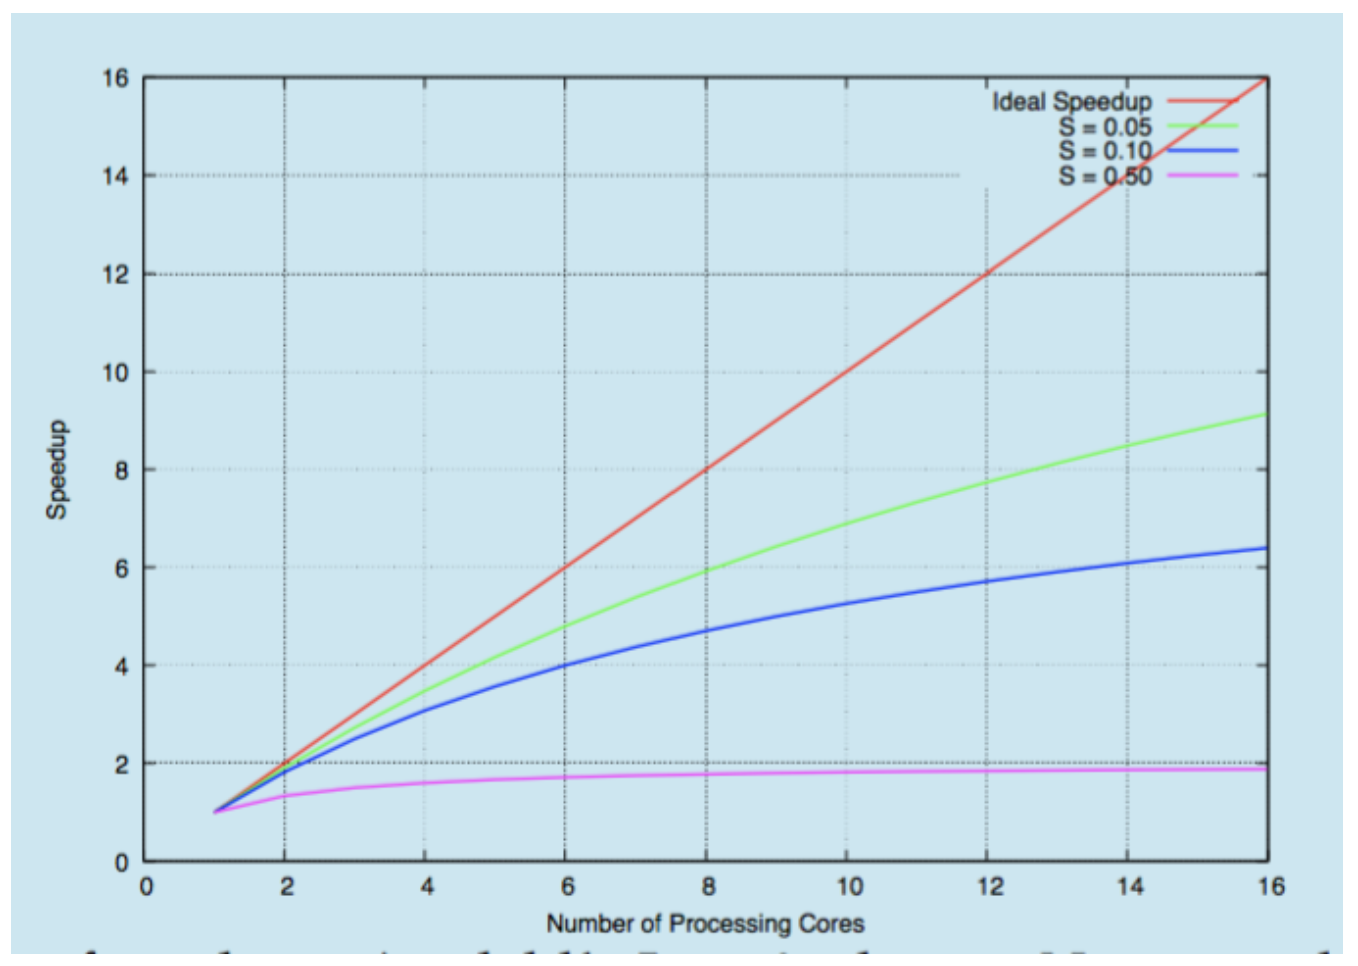
\includegraphics[width=0.75\textwidth]{ambdahl}
\end{center}
Idealmente l'incremento dovrebbe essere esponenziale, ma in realtà si dimostra
che progressivamente si appiattiscono le prestazioni ed il rapporto tra costo
e prestazione diventa meno conveniente.\\ \\
Quindi, si dimostra che più di 4/8 core PER ORA siano più che sufficienti per 
quelle che sono le operazioni che facciamo noi oggi.
\section{Modelli di supporto per Threading}
\begin{itemize}
	\item Thread livello utente:
	Ci sono una serie di librerie in grado di gestire i thread nello spazio 
	dedicato ai processi utente. (Threads di tutto ciò che non è l'OS, per 
	semplificare)
	\item Thread livello Kernel: Tutto ciò che è riguardante l'OS, ad esempio
	il Thread di gestione dell'orologio, oppure quello che serve per anche solo
	la barra applicazioni. \\
\end{itemize}
Inizialmente il kernel era monoThread, e tutto ciò che era multiThread era 
nell'userspace, quindi questo è praticamente pseudoparallelismo, perchè se un
Thread fa I/O allora tutti gli altri staranno in attesa, non è in grado di 
sfruttare più core.\\ \\
\subsection{Modello 1 a 1 } Per ogni Thread del kernel esiste un Thread 
nell'userspace, il che significa che si può sfruttare il parallelismo MA
attenzione.
\\ \\
Se ho un server avente più utenze, se ogni volta tipo 100 utenti mi aprono 
10 Thread a testa, il kernel mi va a 1000 Thread. Per ipotesi si è posto
un limite ai Thread che puoi aprire
\subsection{Modello molti a molti}
Si hanno $\kappa$ Thread del kernel $\times$ $\lambda$ Thread utente, in cui
$\kappa < \lambda$
\section{POSIX PThreads}
Non è un'implementazione ma una specifica (uno standard praticamente) che
consente a sistemi operativi Unix based o anche agli Unix like di poter 
implementare dei Thread. (In c c'è la libreria pThread.h che serve a questo)\\ \\
Su Windows c'è windows.h che consente di avere i Windows Thread, dovrebbero
funzionare anche lì ma in modo più... Minuzioso (No, non dirò quella parola.).
\\ \\
Windows per ogni Thread crea un handle, che va creato e chiuso dal padre del 
Thread.
\section{Thread in Java}
Si possono sviluppare in due modi
\begin{itemize}
	\item Estendendo la classe Thread e creando il metodo run
	\item Implementando l'interfaccia Runnable e anche lì creando il metodo run
	\item Da qui basta instanziare un oggetto di questa vostra classe, e fare
	nomeOggetto.start(); ed il Thread partirà.
\end{itemize}
\section{Threading implicito}
Delega tutto ciò che è la creazione e gestione dei Thread ai compilatori ed 
alle librerie, perchè così gli sviluppatori non devono preoccuparsi di stare
a gestire appunto fattori come chiusura e manutenzione del Thread aperto
\section{Thread pools}
All'avvio viene creato un buon numero di Thread, organizzati in un gruppo che 
semplicemente aspettano di rispondere ad una richiesta, ed in questo modo:
\begin{itemize}
	\item Si accelerano i tempi
	\item Il numero di Thread contemporaneamente aperti è limitato dalla dimensione
	del pool
	\item Separa il task dalla meccanica della sua creazione, avendo o meglio,
	permettendo diverse strategie di esecuzione, con uno scheduling temporale
	nella mia applicazione.
\end{itemize}
Nel POSIX queste meccaniche non ci sono, mentre ci sono su Windows e Java sono
previste
\section{Fork-join}
Vi ricordate il merge sort che divideva in due l'array, no? Ecco, dividiamo
i due array, avviamo un thread per una metà, ed un altro per l'altra metà,
con poi il "combine" vengono riunite.
\section{Problematiche possibile}
Una fork dovrebbe duplicare solo il thread chiamante o tutti i thread in assoluto?
Ecco, il magico mondo UNIX utilizza due tipid i fork per risolvere questa cosa\\ \\
L'exec invece di solito sostituisce tutti i thread del processo
in esecuzione
\section{Signal Handler}
Un segnale è un meccanismo nei sistemi Unix ed Unix like per notificare un evento
ad un processo. \\ \\
Banalmente sono degli interrupt MA lato utente. Ci sono tante scuole di pensiero,
su Unix se hai un segnale verso un processo, allora l'handler viene eseguito
una sola volta, quindi viene eseguito ad un solo thread. Sotto Unix c'è un modo
per fare in modo che un Thread rifiuti un determinato insieme di segnali\\ \\
Un segnale potrebbe essere ctrl+c, che non copia eh, termina l'esecuzione del
programma corrente su terminale .\\ \\
Su Windows non ci sono i segnali ma le APC, che son comunque simili, praticamente
sono delle chiamate di procedura, che sono associate al thread, non al processo.
\section{Cancellazione del thread}
E' possibile fare in modo che un Thread termini l'esecuzione PRIMA che abbia 
effettivamente finito di fare quel che deve fare? Si in due modi
\begin{itemize}
	\item Cancellazione asincrona: Il thread viene terminato di cattiveria, 
	tipo come agli esami a tempo fatti su pc, quando finisce, finisce.
	\item Cancellazione differita: Se thread A vuole terminare B allora B gli
	dice "Spetta n'attimo", e appena finisce si chiude, come quei 5 minuti in 
	più che a volte si riescono a chiedere per finire di scrivere nome cognome
	e data in un esame.. E matricola
\end{itemize}
\chapter{Scheduling della CPU}
\section{Cos'è lo scheduling?}
Schedulare significa stabilire l'ordine e il momento dell'esecuzione delle 
istruzioni impartite a un elaboratore: Cioè per esempio, anche la stampa
di un file.
\paragraph{Osservazione: }Non esiste un solo metodo per schedulare i processi,
infatti esistono svariati algoritmi, addirittura Linux nel corso degli anni
ha cambiato 3 volte i suoi algoritmi
\paragraph{Esiste uno scheduling perfetto? }All'atto pratico no, nel senso, si
deve simulare un ipotetico carico medio di lavoro, per capire come fare 
funzionare al meglio le risorse, ma non esiste l'algoritmo perfetto. SE PERO'
conoscessimo perfettamente il carico di lavoro, ALLORA chiaramente si può
distribuire perfettamente il carico. (Spoiler: No, non si può conoscere 
in modo perfetto.)
\section{Concetti fondamentali}
L'obbiettivo è sempre lo stesso, ovvero massimizzare l'uso della cpu, ed infatti
gli algoritmi di scheduling sfruttano il fatto che di norma l'esecuzione di un 
processo è una serie di \begin{itemize}
\item Burst della CPU: Sequenza di operazioni della CPU
\item Burst dell'I/O: Attesa del completamento dell'operazione di I/O
\end{itemize}
Sapersi gestire i burst della CPU è essenziale. Ma quanto dura un burst?
In programmi normali è generalmente c'è un alto numero di burst brevi ed un 
basso numero di burst lunghi.
\section{Scheduler della CPU (A breve termine)}
Seleziona un processo tra quelli nella ready queue ed alloca un intero core ad 
esso, ma in che modo?
\paragraph{Modo nonPreemptive} o cooperativo, senza preselezione
\begin{enumerate}
	\item Quando un processo passa da running a waiting
	\item Quando un processo passa da running a ready
	\item Quando un processo passa da waiting a ready
	\item Quando un processo termina
\end{enumerate}
Questo metodo è stato praticamente mollato da Windows 95, però non è del tutto
così. Nel senso, Windows 95 eseguiva sia software a 32 che 16 bit, e quindi
quando eseguiva quelli a1 16 utilizzava il metodo nonPreemptive.  
\paragraph{Modo preemptive}
Si applica per rispondere e risolvere le seguenti domande
\begin{enumerate}
	\item E se due processi condividono dati?
	\item E se un processo esegue codice in modalità kernel?
	\item E se un processo sta eseguendo un gestore degli interrupt?
	\item (E se sti gran $^{*}Censura^{*}$ ;) )
\end{enumerate}
\section{Dispatcher}
Si occupa di passare il controllo della CPU al processo scelto dallo scheduler,
e impiega del tempo, infatti esiste un dispatch lag, o anche latenza di dispatch,
che in pratica si genera dalle seguenti operazioni:
\begin{enumerate}
	\item Effetta il cambio di contesto
	\item Passa in modalità utente
	\item Salta nel punto corretto del programma del processo selezionato, cioè
	alla fine dove era stato interrotto
\end{enumerate}
\section{Gli algoritmi di scheduling}
Prima di capire se un algoritmo è migliore di un altro abbiamo da tenere in 
considerazione ci sono una serie di criteri da tenere in considerazione, cioè
\begin{enumerate}
	\item Utilizzo della CPU (In percentuale), quanto tengo impegnata la cpu
	ad eseguire codice utente (Di solito si va dal 40 al 90\%) 
	\item Throughput: Numero di processi che completano l'esecuzione in una
	determinata unità di tempo (ad esempio $\lambda \frac{Processi}{s}$ )
	\item Tempo di completamento: Tempo che serve per finire l'esecuzione
	di un processo (dipende da troppi fattori, tra l'altro c'è pure l'attesa I/O,
	cioè immaginatevi un programma che fa un input e l'utente sta li fermo
	per 3 ore... Ed il programma finisce con print("ciao"))
	\item Tempo di attesa: Tempo in cui il processo sta nella ready queue
	\item Tempo di risposta: Negli ambienti time-sharing (quelli in cui si ha
	un solo core per intenderci) è il tempo che passa da quando arriva una
	richiesta al processo a quando effettivamente si arriva alla prima risposta
	SENZA l'emissione di questa nell'output. %rédichiù
\end{enumerate}
\subsection{Scheduling in ordine d'arrivo}
FCFS (First come, first served), il primo che arriva è il primo che se ne va, 
come le code, sì, esatto. Proprio per questo è anche semplice da implementare,
è una coda.. La sappiamo fare MA ha uno svantaggio, il tempo medio di attesa
(dipendente da quanti processi si hanno) potrebbe essere lungo.
\subsection{Scheduling per brevita}
SJF (Shortest job first), colui che ha il burst più piccino viene preso per primo,
in questo modo diminuisce il tempo di attesa medio.. Ok ma, come fai a sapere 
quanto sarà lungo un burst prima di eseguirlo? Come fai a capire quanti anni ci
avrai impiegato per laurearti PRIMA di avere fatto l'iscrizione in uni? Esatto,
minimo 5 (per la triennale).
\paragraph{Si ma quindi è applicabile?} Allora, fondamentalmente è utopistico ma
applicabile in qualche strano modo, in cui si fanno delle previsioni. Per capire
meglio si fa una stima di durata del burst ragionando sui seguenti dati:
\begin{enumerate}
	\item $T_{n} = $ durata dell'n-esimo burst
	\item Scegliamo un valore $\alpha\in (0,1)$
	\item $T_{\kappa + 1} = \alpha\cdot T_{k} + (1- \alpha)T_{k}$
	\item La mia media esponenziale (data da) $T_{n+1}$
\end{enumerate}
C'è anche una versione preemptive, che si chiama shortest-remaining-time-first,
non è buona come la SJF ma ci si avvicina comunque.
\paragraph{E L'$\alpha$?}
E' un valore che si ottiene confrontando la stima del burst precedente con 
l'effettivo vero burst precedente. Generalmente si mette = 0,5 cioè random
va o uno o l'altro. Se fosse 1 o 0:
\begin{itemize}
	\item 1: Non conta il burst precedente
	\item 0: Conta solo il burst precedente %nell'arrédichiù
\end{itemize}
In questo caso teniamo non proprio in considerazione qual è il processo che 
impiega effettivamente meno, ma quello a cui rimane meno roba da fare
\subsection{Scheduling Circolare}
E' il Round Robin, di solito viene combinato ad altri algoritmi, ma fondamentalmente
è quello pià usato, è il classico algoritmo preemptive.
\paragraph{Come funziona? }Ogni processo ha una quantità fissata di tempo che 
sta tra i 10 ed i 100 millisecondi, ed è praticamente come distribuire le
carte a Poker. \\ \\
So con certezza qual è il limite superiore che un processo attenderà, se ci sono
n processi nella ready queue il quanto temporale è q, ed ogni processo
otterrà $\frac{1}{n} $ di tempo di CPU E nessuno di questi aspetterà più di
q(n-1). 
\subparagraph{Che performance ha?}
\begin{itemize}
	\item Se q è alto, tende al FCFS
	\item Se q è basso, ottieni 
\end{itemize}	
Rispetto a SJF ha un tempo medio più alto dal punto di vista del completamento 
ma allo stesso tempo riduce le latenza, ATTENZIONE, migliorando q non si 
implica un miglioramento del tempo di completamento.
\subsection{Scheduling con Priorità}
Ogni processo ha un numero intero che rappresenta la sua priorità, più è basso
il valore, più questo ha priorità appunto.
Può pure essere preemptive, ed ha priorità sui nonPreemptive
\paragraph{E se due processi hanno stessa proprietà? }A quel punto qualsiasi
strategia va bene, dipende dal processo (Linux questo lo gestisce bene). 
Viene eseguito il processo con priorità più alta per primo chiaramente
\paragraph{Sì, ma se ho un processo di bassa priorità? }Potrebbe pure non essere 
mai schedulato, potrebbe morire per \textbf{Stravation}, non viene mai eseguito
\paragraph{Soluzione? }Invecchiamento (Aging), ossia diminuzione progressiva
del valore di priorità (aumento progressivo della priorità)  
\paragraph{CALMI, Precisiamo meglio questa cosa: }IL VALORE che si associa alla
priorità più è alto, più il processo PERDE priorità. Esempio: Priorità 0 viene 
eseguita PRIMA di priorità 1.
\chapter{Livello Data-Link (SECONDO PARZIALE)}
Per questo argomento vi consiglio di guardarvi 
\href{https://www.isistassinari.gov.it/progettodicembre/reti/L2.html#f}{questo sito: }
\paragraph{Per definizione: }
Il livello data-link riceve dati dal livello fisico, ed offre servizio al livello
network.
Il livello 2 (Data Link Layer) si occupa di gestire il collegamento da un pc 
all'altro appartenenti alla stessa LAN (Local Area Network) e' un sistema di 
comunicazione che permette ad apparecchiature indipendenti di comunicare tra 
loro, entro un' area delimitata, utilizzando un canale fisico a velocita' 
elevata e con basso tasso d'errore. \\ \\Altra funzione principale di questo livello 
e' quella di recuperare gli errori trasmissivi: di solito questo avviene mediante 
tecniche di ritrasmissione automatica dei dati che sono stati ricevuti corrotti.
Il protocollo Ethernet appartiene a questo livello.
\section{Media Access Control}
Il concetto di MAC si introduce ragionando sul concetto del "Mezzo condiviso",
introduciamo inoltre l'uso dello Switch, ovvero un dispositivo che consente
di avere più macchine che sfruttino lo stesso mezzo. 
\section{Switch e Hub}
\begin{itemize}
	\item L'hub quando riceve dei dati automaticamente li invia in broadcast 
	a tutti quanti i nodi connessi
	\item Lo switch invece serve per fare in modo che il pacchetto parta da un
	mittente preciso ed arrivi ad un destinatario (connessi allo switch 
	chiaramente)
\end{itemize}
Ora, anche in questo caso siccome a lezione si ha poca chiarezza, lascerò
lo stesso il materiale direttamente proveniente dalle superiori.
AHAHAHAHAH.
\section{Framing}
Il secondo livello forma dei pacchetti dati, detti frame o trama, da far 
viaggiare lungo la dorsale di comunicazione. Il frame e' l'unita' dati 
fondamentale di questo livello. Il livello DataLink incapsula il pacchetto 
proveniente dallo strato superiore (livello 3) in un nuovo pacchetto detto
frame (o trama) al quale aggiunge un header (intestazione) e un tail (coda).\\ \\
Ethernet, Token Ring, FDDI, IEEE 802.11 (WLAN), ATM, TCP/IP's Serial Link 
Interface Protocol (SLIP) e Point-To-Point Protocol (PPP) sono alcune 
tecnologie e protocolli associati al livello 2. Anche il protocollo 
ARP che permette di conoscere l'indirizzo fisico di una scheda di rete 
corrispondente ad un indirizzo IP, appartiene a questo livello. 
\section{Correzione degli errori}
Sapendo che ci sia un flusso di dati di qualsiasi tipo, è normale che ci sia la
presenza di errori, che dipendono da molteplici fattori. Per intenderci 
il collegamento via radio genera molti più errori rispetto al cavo.
\paragraph{Come si rilevano? }Esistono diversi modi per poter andare a capire
se ci son stati errori 
\subsection{CRC (Codici di ridondanza ciclica)}
\paragraph{In invio: }
Hai il messaggio e il polinomio generatore. Al messaggio aggiungi tanti zeri 
quanto è il grado del polinomio generatore. Poi fai lo XOR tra il messaggio 
finale e il polinomio... Arrivi alla fine, e al messaggio iniziale, aggiungi 
il risultato della divisione, con tante cifre quanto il grado del polinomio..
\paragraph{In ricezione: }
Dividi semplicemente, con lo XOR, il messaggio per il polinomio e se trovi 0 è 
tutto OK, altrimenti ci sono stati degli errori di trasmissione.
\subparagraph{Il polinomio: } può essere scritto in due forme, 
in cifre binarie o con le potenze.. Se è in binario è semplicemente una sequenza
(tipo 1011, 1001 ecc.). Se è con le potenze (può essere una cosa del genere
"G(x)=$x^{3}+x+x^{0}$", " G(x)=$x^{3}+x^{0}$" ecc.) lo trasformi in binario 
(rispettivamente 1011, 1001)	
\section{L'indirizzo MAC}
E' un indirizzo composto da 48 bit (6 byte) ASSOCIATO ALLA SCHEDA DI RETE, in 
pratica NON può cambiare, è univoco, ogni schedina ha il suo MAC address, non 
c'è alcuna relazione tra un MAC address e l'altro, non si possono aggregare, nè
localizzazioni geografiche. L'unico modo è scavare l'indirizzo MAC localmente.
\paragraph{All'atto pratico: }Se ho lo stesso MAC in Italia ed uno in America,
a meno che son proprio stronzo, non saranno mai praticamente nella stessa rete.\\
\\AH SI' poi è chiaro che essendo un numerello scritto in un firmware, allora si
può cambiare con qualche arcano particolare ;) 
\section{Gli accessi concorrenti: }
\subsection{Token Ring: }
Si applica su reti a forma di anello, ovvero reti circolari in cui per ogni
nodo c'è un collegamento a precedente e successivo. 
\paragraph{La particolarità di queste reti sta nel fatto che }lo scambio di 
informazioni è regolato dalla trasmissione di uno dei nodi della rete di un 
particolare messaggio (chiamato token) che stabilisce quale nodo abbia “diritto
di parola” e quale nodo debba ricevere il pacchetto dati (o i pacchetti dati) 
che viaggiano in simbiosi con il token stesso. 
\subparagraph{Come funziona Token Ring: }
All'interno di una LAN organizzata nel modo appena descritto, ogni nodo avrà 
“diritto di parola” sequenzialmente e solo in quel momento sarà autorizzato a 
inviare i suoi pacchetti dati verso il nodo mittente.	
\subparagraph{In modo più specifico: }Pacchetti dati vuoti (detti frame) 
circolano all'interno della Token ring in maniera continua. Quando un computer 
dovrà inviare un messaggio, crea il token contenente i dati del nodo di 
destinazione e lo “lega” ai pacchetti da inviare. Arrivato il suo turno passa 
token e informazioni al computer successivo, che scansiona il token e verifica
quale siano i dati scritti al suo interno; 
\paragraph{}
nel caso in cui non sia lui il 
destinatario della comunicazione, passa pacchetti dati e token al nodo 
successivo. Questa operazione si ripete per ogni nodo della LAN, sino a quando 
il messaggio non raggiunge il suo destinatario. 
\paragraph{}
A questo punto il computer 
copierà i pacchetti dati e sovrascriverà le informazioni presenti nel token,
azzerandolo di fatto. Quando il token avrà completato il proprio giro, il
nodo-mittente scansionerà il “testimone”, 
\paragraph{}
verificherà che le informazioni 
contenute al suo interno sono state sovrascritte ed eliminerà i pacchetti 
dati presenti all'interno del messaggio. All'interno della LAN ad anello 
tornerà a circolare un frame vuoto.	
\subsection{Slotted Aloha: }	
La chiave sta nel fatto di aver individuato il conflitto, e qui si capisce
\end{document}